\section{Comunicação por meio da Luz Visível} \label{sec:comunacaçaoluzvisivel}

Para estudo das principais técnicas de posicionamento empregadas para VLP, é importante retomar a tecnologia que a originou, a VLC. E, compreender os parâmetros fundamentais dos dispositivos envolvidos que serão aplicados na modelagem das técnicas de posicionamento. Os dispositivos eletrônicos de iluminação de estado sólido denominados LEDs, hodiernamente popularizados para utilização em larga escala, têm uma versátil aplicação permitindo o desenvolvimento da VLC, devido a uma de suas características principais, o tempo de resposta. Esses dispositivos podem ser modulados em frequências até na faixa de centenas de milhares de oscilações por segundo, frequências a partir de 200Hz são recomendadas para modulação sem efeitos prejudiciais à visão humana, permitindo o cumprimento do propósito de iluminação e comunicação pelo mesmo dispositivo.

Outro parâmetro a ser considerado diz respeito às frequências eletromagnéticas emitidas pelos LEDs. Esse parâmetro é principal para a escolha dos receptores para cada aplicação. Sua escolha para VLC deve ser feita se considerando- a sensibilidade do sensor utilizado face ao espectro emitido pela fonte de luz, que por sua vez deve considerar o espectro visível humano e o propósito da aplicação dessa iluminação. A Figura~\ref{1} mostra o espectro de emissão dos principais LEDs brancos do mercado. Sendo estes utilizados para diferentes aplicações (as curvas mostram que os sensores teriam diferentes respostas à uma mesma intensidade e posição de luz, devido à diferença no espectro emitido).

\begin{figure}[!h]
    \centering
    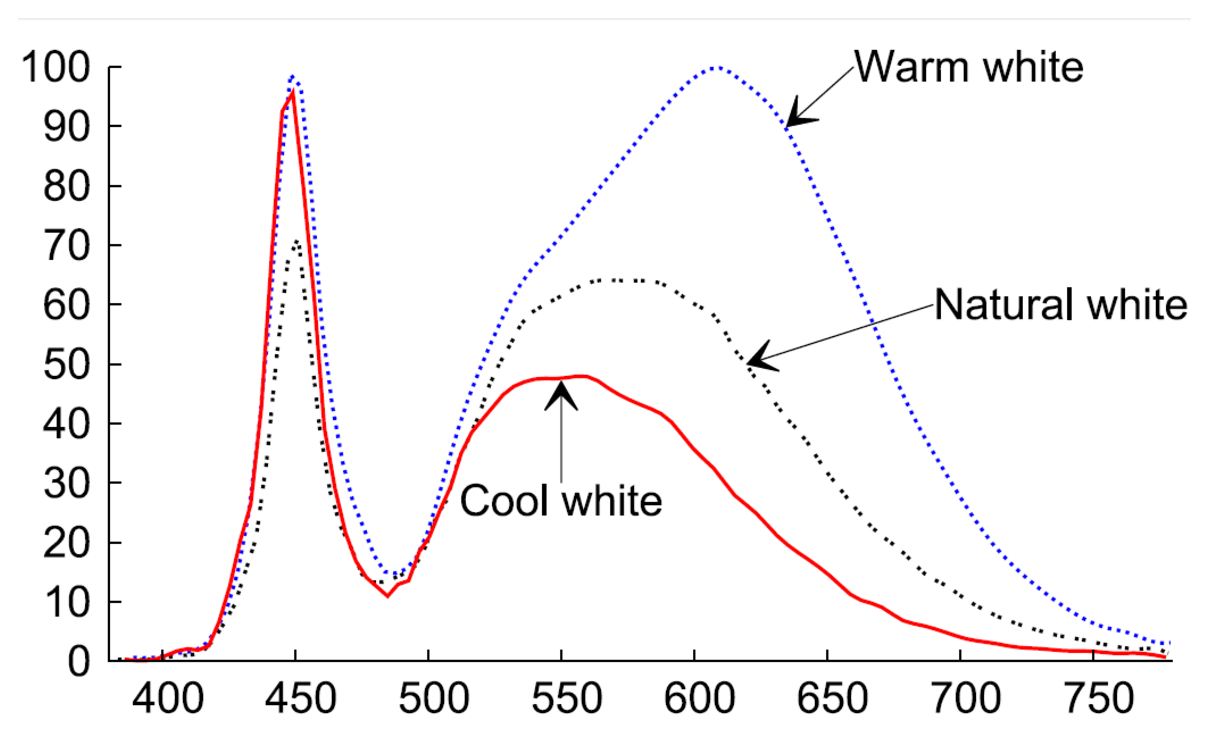
\includegraphics{FIGURA1}
    \caption{Espectro de emissão de LEDs de três cores: Branco frio, Branco natural e Branco quente, mais comumente empregados na iluminação artificial (Imagem retirada de~\cite{7239528})\footnote{Na figura, a abscissa representa o comprimento de onda eletromagnética emitida (em nanômetros) e a ordenada a potência de radiação normalizada (em porcentagem), para LEDs branco quente (linha pontilhada), branco natural (linha tracejada) e branco frio (linha contínua).}.
    \label{1}
\end{figure}
